\documentclass[10pt,a4paper]{article}	
\usepackage{amsmath}
\usepackage{amsfonts}
\usepackage{amssymb}
\usepackage{cite}												% 支持引用多篇文献
\usepackage{CJK}													% 支持中文
\usepackage{indentfirst}                 						% 首行缩进宏包
\usepackage{graphicx}											% 支持图片的插入
\usepackage{subfigure}											% 支持插入子图
\usepackage[colorlinks,citecolor = blue, linkcolor=blue,hyperindex,CJKbookmarks]{hyperref}	% 链接功能
\usepackage{fancyhdr}											% 添加页眉

\graphicspath{{figs/}}                              				% 图片文件夹路径
\setlength{\parindent}{2em}										% 缩进距离为2个字符位置
\newcommand{\song}{\CJKfamily{song}}     						% 宋体
\newcommand{\hei}{\CJKfamily{hei}}       						% 黑体
\newcommand{\fs}{\CJKfamily{fang}}         						% 仿宋
\newcommand{\kai}{\CJKfamily{kai}}       						% 楷体
\newcommand{\li}{\CJKfamily{li}}         						% 隶书
\newcommand{\you}{\CJKfamily{you}}       						% 幼圆


\begin{document}

\begin{CJK*}{UTF8}{gkai}
%============================++题目和作者++================================
\title{关于人形机器人的调研报告}					   							% 题目
\author{郝俊禹\thanks{Email:haojunyu2012@gmail.com}}				% 作者
%============================++++++++++++=================================
\date{}                                             				% 显示作者,不显示日期
\maketitle                                          				% 生成标题
\tableofcontents 												% 生成目录
\clearpage


\section{引言}
随着信息时代的到来,机器人技术的发展是个必然的趋势。 机器人的出现并高速发展是社会和经济发展的必然,是为了提高社会的生产水平和人类的生活质量。 

人形机器人的出现是计算机科学、传感器技术、机械科学等学科的技术进步,也是人类日常生活需要的产物。关于它的研究起步于1960年代后期,主要目的是解决人形机器人的双足行走问题。进入1990年代后,人形机器人在控制方法和人工智能等方面的研究成果不断出现,从而推动了人形机器人技术的快速发展,此后机器人的行走能力、智能化和功能都越来越强大。



\section{人形机器人的相关概念及历史}
\subsection{人形机器人的定义及分类}
人形机器人,又称拟人机器人(humanoid),指是以模仿真人作为目的制造的机器人,大小上可以和真人差很远,也可以没有似人的外观,但有人的四肢和头等构造。\cite{1}

对于人形机器人的分类主要有以下几种\cite{2}:
\begin{description}
\item[拟人智能机器人(HIR)] 具有拟人智能的机器人,例如具有自行制定行为规划能力的机器人
\item[拟人情感机器人(HEmR)] 具有拟人情感的机器人,例如能与人进行情感交流的机器人
\item[拟人进化机器人(HEvR)] 具有自学习、自进化能力的机器人
\item[拟人行为机器人(HBR)] 例如步行机器人,舞蹈机器人,足球机器人等
\item[拟人形象机器人(HFR)] 具有拟人外观形象的机器人,例如虚拟电视节目主持人、电影演员、游戏角色
\item[拟人构造机器人(HAR)] 具有拟人内部构造的机器人,例如具有拟人内部器官组织构造,用于人体生理解剖,医学教学何研究的机器人
\end{description}

\subsection{典型的人形机器人}
\subsubsection{ASIMO}
ASIMO(日语:アシモ)是日本本田技研工业所开发的可双足自律行走的人形机器人。ASIMO外型酷似一位背着背包的太空人,外形如图\ref{fig:ASIMO}。\\
\begin{figure}[!htbp]
	\centering
	\caption{ASIMO}  
		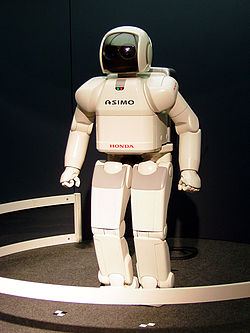
\includegraphics[scale=0.30]{figs/HONDA_ASIMO.jpg}
    	\label{fig:ASIMO}
\end{figure}


ASIMO已经可以同时与多人进行对话;
能够以时速9公里的速度前进,遭遇其他正在行动中的人时,会预测对方行进方向及速度,自行预先计算替代路线以免与对方相撞;
腿部的运动能力及活动范围不仅可以步行、奔跑、倒退走,还可以单脚跳跃、双脚跳跃,更能边跳跃边变换方向,也可以在一些微不平的地面行走;
手部可转开水瓶、握住纸杯、进行倒水,手指动作更纤细,甚至可以边说话边以手语表现说话内容。


\subsubsection{NAO}
NAO (发音和 Now 相近) 是一个自主的可编程仿人机器人,由法国Aldebaran机器人公司研发。外形如下图\ref{fig:NAO}。\\
\begin{figure}[!htbp]
	\centering
	\caption{NAO}  
		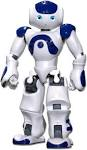
\includegraphics[scale=0.40]{figs/NAO.jpg}
    	\label{fig:NAO}
\end{figure}

NAO具有两个不同定位的版本:学术版(售价两万欧元)与家庭版。NAO家庭版面世较早,面向个人、家庭、服务行业,用于互动娱乐。NAO学术版面向大学和实验室,用于科学研究和教学。

NAO机器人拥有着讨人喜欢的外形。并具备有一定程度的人工智能和约一定程度的情感智商并能够和人亲切的互动。该机器人还如同真正的人类婴儿一般拥有学习能力。它可以通过学习身体语言和表情来推断出人的情感变化,并且随着时间的推移“认识”更多的人,并能够分辨这些人不同的行为及面孔。并且能够表现出愤怒、恐惧、悲伤、幸福,兴奋和自豪的情感。当它们在面对一个不可能应付的紧张状况时,如果没有人与其交流,NAO机器人甚至还会为此生气。它的“脑子”可以让它记住以往好或坏的体验经验。

\subsubsection{Actroid-DER系列}
Actroid是一个与人非常类似的,由Osaka大学开发,KOKORO有限公司制造的人形机器人。外形如图\ref{fig:actroid}。\\
\begin{figure}[!htbp]
	\centering
	\caption{ACTROID}  
		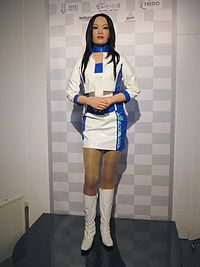
\includegraphics[scale=0.35]{figs/Actroid.jpg}
    	\label{fig:actroid}
\end{figure}


它可以模仿人类类似的行为,比如眨眼睛,说话,呼吸等,具有识别和处理的能力她可以演讲并应对实物,是一个互动的机器人。


\subsection{人形机器人的研究进度}
在人形机器人研究方面,我国也作了很多工作。国防科技大学、哈尔滨工业大学研制出了双足步行机器人,北京航空航天大学、北京科技大学研制出了多指灵巧手等。他们主要的研究大方向如下。
\begin{enumerate}
\item 人形机器人步行控制方面\\
文献\cite{3}通过针对人形机器人的控制难点:关节扭矩不够,运动稳定性不佳等方面,运用许多控制理论,如倒立摆,zmp,虚拟斜坡,被动步态等,最终实现了仿真平台下人形机器人的稳定行走。


文献\cite{4}通过仿真来研究、分析和检验仿人形机器人在步行过程中的受力,改进和提高了人形机器人的步行控制方法。
\item 人形机器人语音识别方面\\
文献\cite{5}通过利用人形机器人具有的类似人体的头相关传输函数的性质,结合自适应滤波方法,对基于空间信息的方法进行扩展:对一路或多路阵元采集的信号按信道间差异特性进行处理,降低其与目标声源方向原始声音信号的相关性,得到与目标信号弱相关的参考噪声,然后进行自适应滤波,得到对目标信号的实时估计。

文献\cite{6}通过Agent技术的语音识别网络的构建,实现让机器人对外界语音输入能够正确地识别和理解,为机器人进一步进行情感上的交流奠定基础。
\end{enumerate}


\section{相关智能机器人的简介}
\subsection{情感机器人}
情感机器人是赋予了人类式情感的机器人,具有表达、识别和理解喜乐哀怒的能力。
\begin{itemize}
\item 2010.08.10 欧洲研发首个能表达情感机器人nao可以模仿1岁孩童的情绪并可以与善意对它的人结下深情厚谊
\item 2012.02.02 荷兰科学家研发情感机器人可表达喜怒哀乐。
\item 2013.01.18 合肥工业大学研制出情感机器人,能陪聊天逗开心
\end{itemize}
文献\cite{7}通过建立仿人类情感的情感模型,在情感模型中建立了三维情感空间,采用马尔可夫过程来描述情感状态的变化转移过程,并提出了性格矩阵,对比分析了不同性格人对相同刺激的反应。

\subsection{认知机器人}
认知机器人是一种具有类似人类的高层认知能力,并能适应复杂环境,完成复杂任务的新一代机器人。目前对于认知机器人的理解以及具体的方法与实现包括认知机器人架构,学习方法,记忆系统,内部机制等方面。认知机器人的研究分为三个基本问题:学习问题,发育问题,决策问题。


文献\cite{8}将模糊逻辑引入到设计中,利用两个模糊控制器控制一个机械臂与另一个传统工业机械臂配合,平稳地抬起一个物品,并利用MATLAB软件进行了仿真实验。使机器人能够通过一个主动探索和收集信息的过程对用户的意图和喜好进行认知。

\section{总结}
\subsection{购买情况}
在上面的三个比较有名气的人形机器人中,ASIMO未提供出售信息,NAO的学术版售价20000欧元,actroid-der系列提供只能以出租的方式被引进。


		
		
\bibliographystyle{unsrt}										% 按引用的先后顺序排列,比较次序为作者,年度和标题
\bibliography{mybib}												% 引用文件数据库在bib.bib文件中

\clearpage     
\end{CJK*}
\end{document}
